\section{Auswertung}
\label{sec:Auswertung}
Zur Berechnung des Mittelwerts $\overline{x}$ einer Größe mit $n$ Messungen der Größe $x$ wird die Formel 
\begin{equation}
  \overline{x}=\frac{1}{n}\sum_{i=1}^n x_n,
  \label{eq:Mittelwert}
\end{equation} verwendet.
Die dazu gehörige Standardabweichung $\sigma$ ergibt sich über 
\begin{equation}
  \sigma=\sqrt{\frac{1}{n-1}\sum_{i=1}^n(x_n-\overline{x})^2}
  \label{eq:Standardabweichung}
\end{equation}
Zum Berechnen der Fehler wird die Gaußsche Fehlerfortpflanzung genutzt 
\begin{equation}
\increment f=\sqrt{\sum_{k=1}^{n}\biggl(\frac{\partial f}{\partial x_\text{k}}\biggr)^2(\increment x_\text{k})^2}\,.
\label{eq:gauss}
\end{equation}
Dabei ist $f$ die zur Berechnung der Größe gegebene Formel und $x_k$ dessen Argumente.
$\increment x_k$ ist der jeweilige Fehler der einzelnen Argumente.
Zunächst wird aus den Messwerten die Winkelrichtgröße $D$ bestimmt.
\begin{table}[H]
  \centering
  \caption{Messwerte zur Bestimmung der Winkelrichtgröße}
  \label{tab:Winkelrichtgroesse}
  \begin{tabular}{
  c c
  }
    \toprule
     $\phi \, / \unit{°}$ & $F\, / \unit{\newton}$\\
    \midrule
    110 & 0.21 \\
    100 & 0.19 \\
    90  & 0.188\\
    80  & 0.168\\
    70  & 0.147\\
    60  & 0.118\\
    50  & 0.090\\
    40  & 0.060\\
    30  & 0.038\\
    20  & 0.016\\
    \bottomrule
  \end{tabular}
\end{table}
Hierfür werden die Drehwinkel $\phi$ zu nächst von $^\circ$ in $rad$ umgerechnet, 
was mit $\phi_\text{neu} = \sfrac{\phi \pi}{180}$ durchgeführt wird.
$D$ wird daraufhin mittels
\begin{equation}
  D = \frac{F R}{\phi_\text{neu}}
\end{equation}
bestimmt.
Dabei ist $F$ die gemessene Kraft und $R$ der Radius, an dem der Kraftmesser befestigt wird.
In diesem Versuch wird $R = \SI{0.2}{\meter}$ gewählt.
Es werden die Winkelrichtgrößen aller Winkel einzeln ausgerechnet.
Anschließend wird der Mittelwert und die Standartabweichung dieser gebildet und die Winkelgröße
\begin{equation*}
  D = \SI{0.01997 \pm 0.00466}{\N \meter}
\end{equation*}
ergibt sich.

Zur Auswertung der Daten in Tabelle \ref{tab:Traegheitsmoment},

\begin{table}[H]
  \centering
  \caption{Messwerte zur Bestimmung des Trägheitsmoments}
  \label{tab:Traegheitsmoment}
  \begin{tabular}{
  c c
  }
    \toprule
     $R \, / \unit{\meter}$ & $F\, / \unit{\newton}$\\
    \midrule
    0.05  & 14.16 \\
    0.075 & 15.97 \\
    0.10  & 18.34 \\
    0.125 & 20.78 \\
    0.15  & 23.47 \\
    0.175 & 26.47 \\
    0.20  & 29.81 \\
    0.225 & 32.81 \\
    0.25  & 35.82 \\
    0.30  & 41.79 \\
    \bottomrule
  \end{tabular}
\end{table}
\begin{figure}[H]
  \centering
  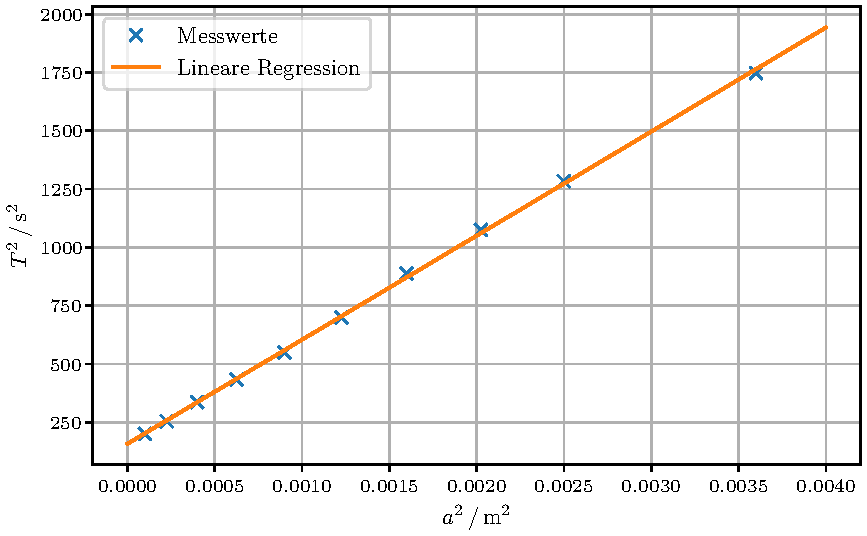
\includegraphics[scale=0.6]{Python/plotI_D.pdf}
  \caption{Das Quadrat des Abstandes aufgetragen gegen das Quadrat der einfachen Schwingungsdauer.}
  \label{fig:Plot1}
\end{figure}



\begin{table}[H]
  \centering
  \caption{5-fache Schwingungsdauer einer Kugel und einers Zylinders}
  \label{tab:Kugel_Zylinder}
  \begin{tabular}{
  c c
  }
    \toprule
     $T_\text{Kugel}\, / \unit{\second}$ & $T_\text{Zylinder}\, / \unit{\second}$\\
    \midrule
    9.15 & 9.47 \\
    9.31 & 9.43 \\
    9.19 & 9.31 \\
    9.34 & 9.47 \\
    9.28 & 9.31 \\
    9.35 & 9.28 \\
    9.41 & 9.41 \\
    9.28 & 9.31 \\
    9.31 & 9.28 \\
    9.35 & 9.28 \\
    \bottomrule
  \end{tabular}
\end{table}
\subsection{Trägheitsmoment einer Kugel}


\begin{table}[H]
  \centering
  \caption{Schwingungsdauer einer Kugel für eine Auslenkung von $90°$.}
  \label{tab:Kugel}
    \begin{tblr}{
      colspec={c|c}
      }
    \toprule
    $t$ / s & $t$ / s\\
    \midrule
    1.83 & 1.87\\
    1.86 & 1.88\\
    1.84 & 1.86\\
    1.87 & 1.86\\
    1.86 & 1.87\\
    \bottomrule
    \end{tblr}
\end{table}
Die verwendete Holzkugel hat die Masse $M_\text{K}=\SI{1172.6}{\gram}$ und den Radius $R_\text{K}=\SI{7.34}{\centi\meter}$. 
Mittels Gl. \eqref{eq:Mittelwert} und \eqref{eq:Standardabweichung} ergibt sich aus den Daten der Tabelle \ref{tab:Kugel} 
eine mittlere Schwingungsdauer von $\overline{t}=\SI{1.86\pm0.015}{\second}$.Mit Einsetzen der gemessenen Werte in Gleichung 
\eqref{eq:Kugel} ein ergibt sich ein Theoriewert für das Trägheitsmoment der Kugel von $I_{\text{K,theo}}=\SI{2.53e-4}
{\kilo\gram\meter\squared}$.
Unter Verwendung der Gl. \eqref{eq:Schwingungsdauer} umgestellt nach $I$ ergibt sich
ein experimenteller Wert von $I=\SI{0.161}{\kilo\gram\meter\squared}$.